\documentclass{article}
\usepackage{graphicx}
\graphicspath{ {images/} }
\begin{document}
\title{Office Sale's Database Project}
\author{Daniel Alberto Zarco Manzanares (Project Manager)\\Gabriela Gaytan Medina (Database analyst)\\Omar Hernandez Francisco (Web Developer)\\ Josué David Rivera Arellane (Developer Jr.)\\\\GEANT Consultora S. de R.L. de C.V.\\ 
\includegraphics[width=6.5cm]{EmpresaAdminProyectos}}
\date{May 21, 2020}
\maketitle
\newpage
\section{About us}
\subsection{Daniel Alberto Zarco Manzanares (Project Manager)}
I'm student in computer engineering in Engineering's faculty where, alongside of my student career my focus has been develop all skills oriented to leadership, financial, management and high direction for business. My role since I was started my degree was be a leader of team, have organization and mark direction of projects. I'm really satisfied of be a member or Engineering's faculty.
\subsection{Omar Hernandez Francisco (Web Developer)}
My name is Omar Hernández Francisco, I was born in the State of Mexico, where I attended the primary educational level at the José Martí school, and later entered the secondary educational level at the José Vasconcelos School and finished my Baccalaureate at the Plantel Oriente School of Sciences and Humanities , where I had a robot programming course.
Later he entered UNAM, specifically in the Faculty of Engineering (FI) where he is currently pursuing a degree in computer engineering.
As for work, I started working at the age of 16. This is driven by the training of my mother which stopped me from teaching to be a worker and achieve things through hard work. In this first job I started a job where I was in charge of carrying out a control on the entry of personnel into the establishment. Later, after a year of entering my first job, I entered the Swiss pastry, working as a pastry chef as well as in the dessert area. Already with some experience in different types, I had the opportunity to work in a friend's business, where I was able to obtain knowledge about the production of pizzas, here I lasted about a year working from Monday to Friday, but due to entering my degree I had to leave it.
Due to different changes throughout my career, I currently do not have a formal job, but I took advantage of the free times that sometimes arise to carry out maintenance work on computer equipment.
\subsection{Gabriela Gaytan Medina (Database analyst)}
My name is Gabriela Gaytan Medina and I was born in Mexico City on July 11, 1997; My residence is in the State of Mexico, but I have spent my daily life in the city.
In May 2015, at the age of 17, I finished my Baccalaureate at the Vallejo School of Science and Humanities, processed my regulated pass for the Bachelor of Computer Engineering. Later in August 2015, at the age of 18, I entered the faculty and that career.
In the Faculty of Engineering I have learned different values including responsibility, perseverance, effort, honesty, integrity and respect.
I have participated in different projects, in the semester 2021-1, I participated in the modern digital design contest, which was based on a contest, even though I did not win I learned to work as a team.
My academic life throughout the faculty has been satisfying and a great learning experience.
\subsection{Josué David Rivera Arellane (Developer Jr.)}
Hi, my name is Rivera Arellanes Josue David, born in “Naucalpan de Juarez, Edo Mex”. Like everyone, i’m a student at Faculty of engineering, actually studying computer engineering. 
About my laboral career, i only was in two informal Jobs, like be packer in Wallmart and be assistant at a pizza shop. 
I haven’t a formal job yet, but im thinking in taking someone son for gain experience.
\newpage
\section{Introduction}
GEANT consultora design a simple solution for project, this project has a structure divided by two parts, first part corresponding to Database process planning, an second corresponds to Web process planing.
The project's requirements is design, development and deployment a data base for stationery's business. 
We opted to a simple structure in single computer, optimizing the development process, time and financial estimation. This simple structure is best than client-server structure, is less expensive in time and financial estimation.
\subsection{Structure's description}
Our structure's design has single computer that have dual function, first as server 		where every send request arrive at server. Second function as data base, where 		has stored all information about the business line and internal process.
\begin{enumerate}
\item Server: Server provide stored data of web site, where we can manipulate in simple form all data generated by information's flow. We use server with local area network(LAN).
\item Database: Developed across client's requirements, database can stored all information of business line structure. Client's information, sale's transactions, providers information and complete data around at products. 
\begin{center}
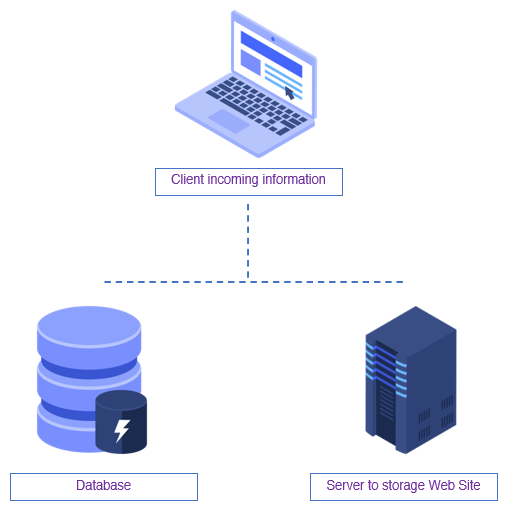
\includegraphics[width=9cm]{structured}
\end{center}
\end{enumerate}
\section{Scheduling plan}
Following scheduling plan has purpose to organize all phases of development process. Cause we had a tight time to development this project, we designed this with high quality and minimum complexity.
\begin{center}
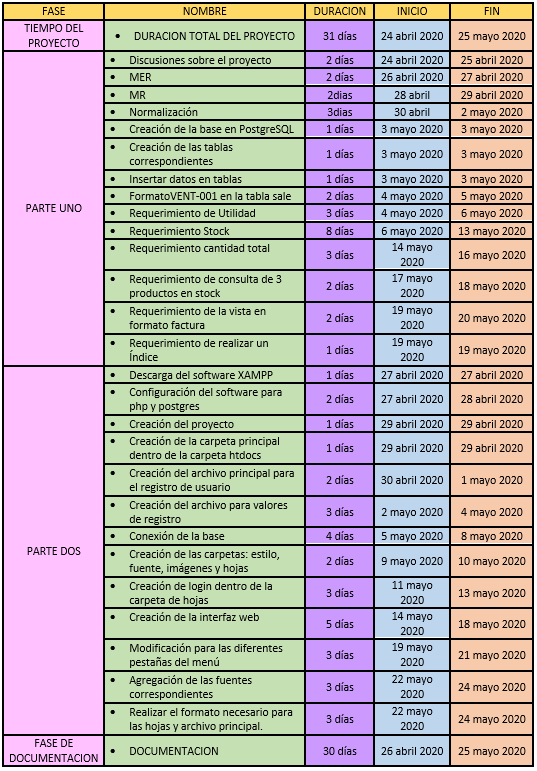
\includegraphics[width=11cm]{cronograma}
\end{center}
Details of scheduling plan
\begin{center}
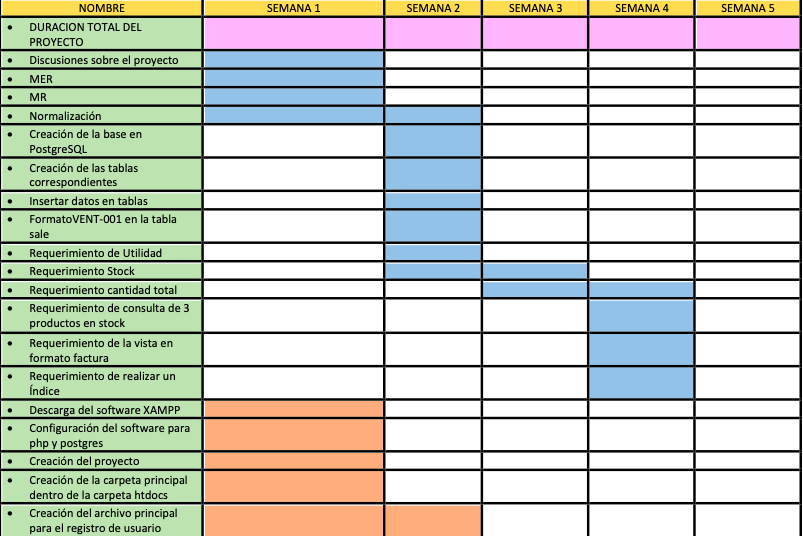
\includegraphics[width=9cm]{crono2}
\end{center}
Next diagram show description of all phases of this project.
\begin{center}
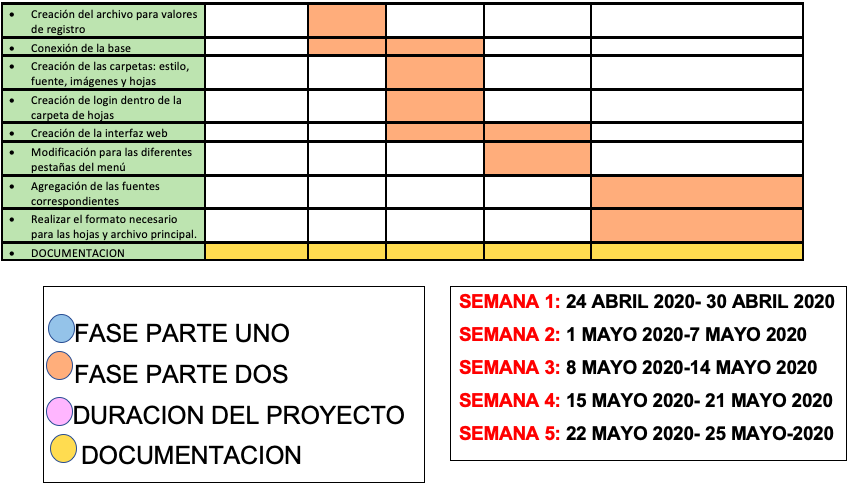
\includegraphics[width=9cm]{crono3}
\end{center}
\section{Design}
\subsection{Requirements}
We took all project's requirements for business line. Following list contain all requirements.
\begin{enumerate}
\item When arrive product's bar code, shows the product's utility.
\item When registered a sale, must decrease the stock if product's stock is greater than 3 pieces, if product's stock is equal 3 pieces, must return a warning notifying to client that stock is equal 3 pieces or less, and if product's stock is zero, notify an error and stop the sale.
\item  Get the product's name which stock is less than three pieces.
\item Generate view to show necessary information to be equal a bill.
\item Create at leas one index and justify the reason to create that index in these place.
\end{enumerate}
\subsection{Design Entity relation model}
Following image, show our entity relation model for set base of database.
\begin{center}
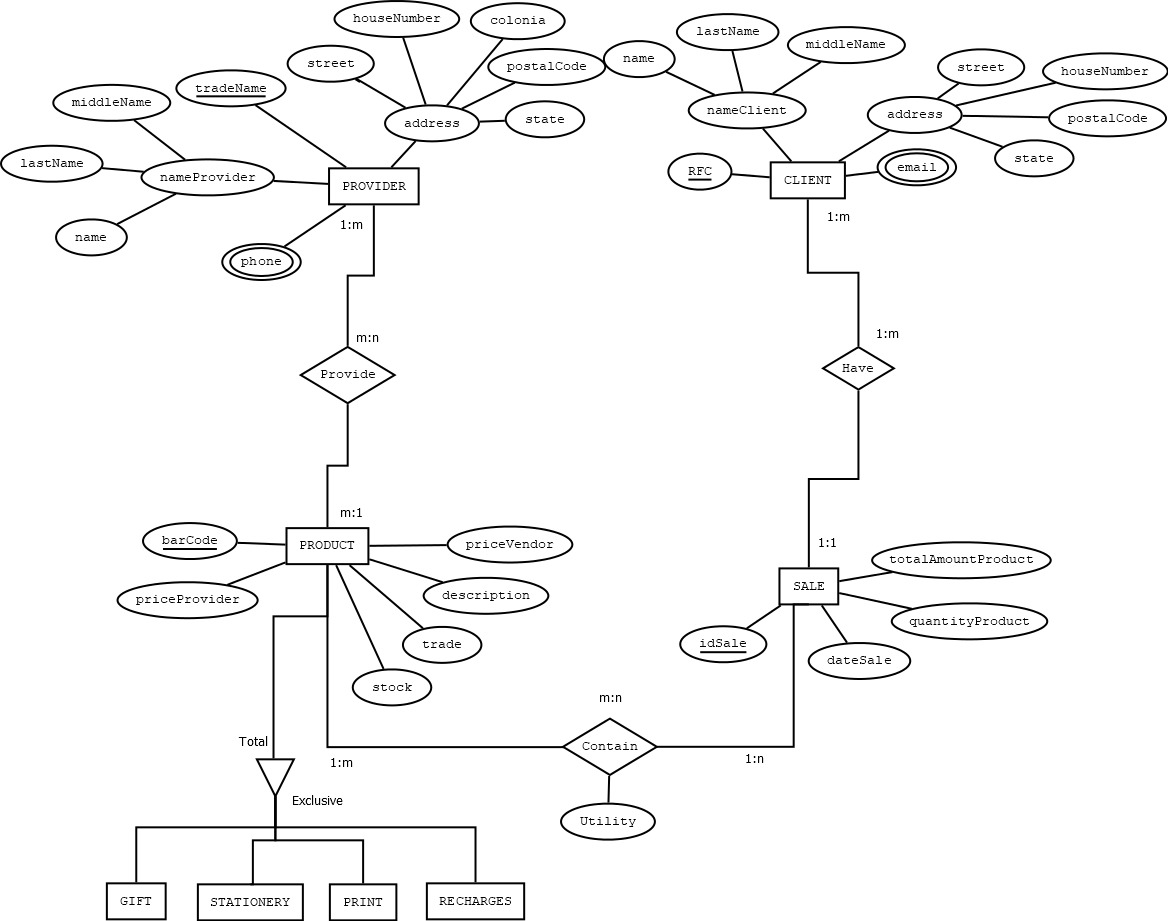
\includegraphics[width=9cm]{OfficeSaleSystemDB_MER}
\end{center}
Diagram shows above have all specifications to describe all data with specific format requires our client , detailed in his requirement document. 
\subsection{Relational model}
Following diagram correspond to third phase, building a relational model diagram, and receive entity relation model document as input.
\begin{center}
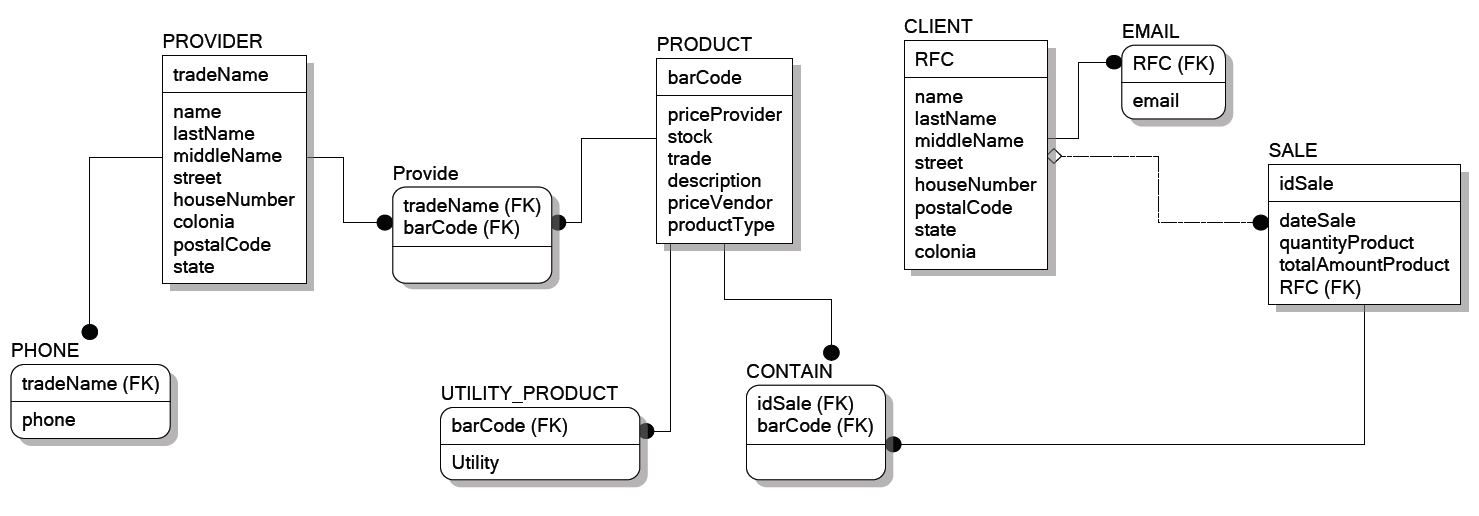
\includegraphics[width=9cm]{mr}
\end{center}
Diagram shows above
\section{Implementation}
To show files of source codes, please check the corresponding folder inside project.
\subsection{Utility by product's bar code}
Implemented by creation of function that returns a table with followings attributes:
\begin{enumerate}
\item Product's bar code
\item Product's trade
\item Product's description
\item Product's utility
\end{enumerate}
Code of implementation: Function return a table with product's attributes to have more information, included the financial utility.
\begin{verbatim}
CREATE OR REPLACE FUNCTION utility(barcode_chose VARCHAR) 
RETURNS TABLE(
    barcode_product VARCHAR,
    trade_product VARCHAR,
    description_product VARCHAR,
    utility_product FLOAT)
AS $$
DECLARE
    price_prov FLOAT;
    price_ven FLOAT;
    utility_net FLOAT;
BEGIN
    SELECT priceprovider INTO price_prov FROM product WHERE barcode=barcode_chose;
    SELECT pricevendor INTO price_ven FROM product WHERE barcode=barcode_chose;
    utility_net= price_ven-price_prov;
    RETURN QUERY SELECT
        barcode,
        trade,
        description,
        utility_net
        FROM 
            product
        WHERE
            barcode=barcode_chose;
END; $$
LANGUAGE 'plpgsql';
\end{verbatim}
\subsection{Updating product's stock while transaction's process is running}
Implemented by trigger, is necessary to execute trigger before to insert sale's data and function inside of trigger checks every product's stock, getting their information through variables. Once function get the values, checks stock and their quantity, if product's stock is greater than three pieces, sale's registration is running normally, when transaction's process is running function checks actual stock, update record and notify if stock is less than three prices. Also function checks if stock is equal to zero, and is it, sale's process is aborted. Every process is running through case validations.
\begin{verbatim}
CREATE OR REPLACE FUNCTION INVENTARIO () RETURNS TRIGGER AS $$
DECLARE
 stock2 INTEGER;
 stock1 INTEGER;
BEGIN
    select stock INTO stock2 FROM product WHERE barcode=new.idproduct;
    stock1=new.quantityproduct;
    RAISE NOTICE 'new idsale: %',new.idsale;
    RAISE NOTICE 'stock1=quantityproduct: %',stock1;
    CASE
        WHEN stock2=1 or stock2<=0 THEN
            RAISE EXCEPTION USING MESSAGE = 'No hay productos en stock.';
        WHEN stock2<=3 THEN
            RAISE WARNING 'Quedan 3 o menos piezas en Stock, stock % pz. - %',stock2, NOW();
            UPDATE product
            SET stock=stock2-stock1
            WHERE barcode=new.idproduct;
        WHEN stock2>3 THEN
            UPDATE product
            SET stock=stock2-stock1
            WHERE barcode=new.idproduct;
            RAISE NOTICE 'Se realizo correctamente la actualización del stock %. stock2 %, stock1 %', now(), stock2, stock1;
        ELSE
            RAISE NOTICE 'Error en actualizar stock';
    END CASE;
    RETURN NEW;
END; $$
LANGUAGE 'plpgsql';

CREATE TRIGGER trstock BEFORE INSERT ON sale
FOR EACH ROW EXECUTE PROCEDURE INVENTARIO();
\end{verbatim}
\subsection{Gets products where stock is less than three}
We implemented in this requirement a function to returns a table with product's information. Below you can find respective code:
\begin{verbatim}
CREATE OR REPLACE FUNCTION checkstock() RETURNS TABLE(
    barcode_checks VARCHAR,
    priceprovider_check FLOAT,
    stock_checks INTEGER,
    trade_checks VARCHAR,
    description_checks VARCHAR,
    pricevendor_check FLOAT,
    product_type VARCHAR
)
AS $$
BEGIN
    RETURN QUERY SELECT
        barcode,
        priceprovider,
        stock,
        trade,
        description,
        pricevendor,
        producttype
        FROM
            product
        WHERE
            stock<3;
END; $$
LANGUAGE 'plpgsql';
\end{verbatim}
\subsection{Generation of bill view}
Implemented by function where this gets as parameter idsale, with this parameters, function sear along table of sale the choose idsale and returns all information about this sale, product, and client and transforms into bill. 
\begin{verbatim}
CREATE OR REPLACE FUNCTION billinfo(IN id_sale VARCHAR)
RETURNS TABLE(
    id_sale_bill VARCHAR,
    barcode_bill VARCHAR,
    description_bill VARCHAR,
    quantityp_bill INTEGER,
    price_vendor_bill FLOAT,
    total_bill FLOAT
) AS $$
DECLARE
total_p FLOAT;
price_prod FLOAT;
quant INTEGER;
idd_sale VARCHAR;
name_bill VARCHAR;
last_name_bill VARCHAR;
rfc_bill VARCHAR;
street_bill VARCHAR;
house_bill VARCHAR;
colonia_bill VARCHAR;
postal_code_bill VARCHAR;
state_bill VARCHAR;
BEGIN
    SELECT c.name INTO name_bill FROM client c 
    INNER JOIN sale s ON c.rfc=s.rfc WHERE idsale=id_sale;
    SELECT c.lastname INTO last_name_bill FROM client c 
    INNER JOIN sale s ON c.rfc=s.rfc WHERE idsale=id_sale;
    SELECT c.rfc INTO rfc_bill FROM client c 
    INNER JOIN sale s ON c.rfc=s.rfc WHERE idsale=id_sale;
    SELECT c.street INTO street_bill FROM client c 
    INNER JOIN sale s ON c.rfc=s.rfc WHERE idsale=id_sale;
    SELECT c.housenumber INTO house_bill FROM client c 
    INNER JOIN sale s ON c.rfc=s.rfc WHERE idsale=id_sale;
    SELECT c.colonia INTO colonia_bill FROM client c 
    INNER JOIN sale s ON c.rfc=s.rfc WHERE idsale=id_sale;
    SELECT c.postalcode INTO postal_code_bill FROM client c 
    INNER JOIN sale s ON c.rfc=s.rfc WHERE idsale=id_sale;
    SELECT c.state INTO state_bill FROM client c 
    INNER JOIN sale s ON c.rfc=s.rfc WHERE idsale=id_sale;

    RAISE NOTICE 'GEANT S. de R.L. de C.V.';
    RAISE NOTICE 'www.geantcommerce.com.mx';
    RAISE NOTICE 'Telephone: 26-45-78-41';
    RAISE NOTICE 'Alvaro Obregón, Ciudad de México.';
    RAISE NOTICE 'Bill to % %',name_bill,last_name_bill;
    RAISE NOTICE 'RFC: %',rfc_bill;
    RAISE NOTICE 'Address: %, %, %, %, %',street_bill, house_bill, colonia_bill, postal_code_bill, state_bill;
    SELECT pricevendor INTO price_prod FROM product INNER JOIN sale ON barcode=idproduct WHERE idsale=id_sale;
    SELECT quantityproduct INTO quant FROM product INNER JOIN sale ON barcode=idproduct WHERE idsale=id_sale;
    total_p=quant*price_prod;
    idd_sale=id_sale;
    RETURN QUERY SELECT
        idd_sale,
        barcode,
        description,
        quant,
        price_prod,
        total_p
        FROM
        product INNER JOIN sale ON barcode=idproduct
        WHERE
        idsale=id_sale;
END; $$
LANGUAGE 'plpgsql';
\end{verbatim}
\subsection{Create index to optimizing searching on database}
Create a index on sale table in column idsale cause table will have  many record with all sales generated in time period.
\begin{verbatim}
create index indiceventa on sale (idsale)
\end{verbatim}
\section{Presentation}
For the connection of our database with the web interface, it was necessary to use the Xampp software, which is a server with Apache distribution which will be in charge of making a connection between the database in Postgresql and php.
To make the connection already having this software, the first thing to do was the Xampp configuration, since it is not configured to work together with postgresql - php. Here's how this configuration is done.
\begin{center}
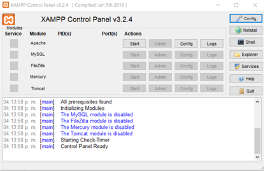
\includegraphics[width=9cm]{xampp1}
\end{center}
Having already made the configuration, we proceeded to test the connection. Having a database ready in postgresql we turn on the Xampp server with Apache. Then we create a folder where our project will be housed, and inside it we create our php file. It should be noted that this folder must be located in the "hdocs" folder, which can be found within the Xampp installation path.
\begin{center}
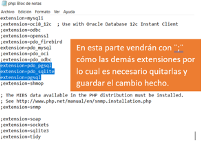
\includegraphics[width=9cm]{xampp2}
\end{center}•
Finally, to call the connection to the desired database, the following syntax is used
\section{Conclusion}
\subsection{Daniel Alberto Zarco Manzanares (Project Manager)}
This project was an interest challenge cause time was very tight. In development phase we had some difficulties in design and planning some requirements. Specially, postgres has an derivate sub language of SQL called plpgsql, where syntax is similar but also complicated. We studying and implemented sql language not plpgsql. In entire project we had a complex requirement, and it was checks stock of an product to verify status of this, following rules given by amount of stock.
Challenge was overcome with success.
\subsection{Omar Hernandez Francisco (Web Developer)}
At the end of carrying out the project, I managed to get a feedback on all the concepts and techniques used throughout the Database course and, nevertheless, I was able to apply them in a work that gives us an overview of the types of problems that we may encounter throughout of our career as professionals.
During the development of the project there were different aspects that were well applied, for example, the fact of having a designated leader to give the different guidelines on how to carry out the elaboration of the work. But as we know not everything goes right the first time, because a great challenge that I could notice was that having to depend on the work that the other team members were working on is a very serious delay on any job, since many times we needed to A certain part of the database was already perfectly made to work based on those results.
A complication that I had in this project was that I had never tried to make a database connection with Postgresql and although there is different information on the web about the software that should be used for the correct connection, it was not enough because the problem was not in Xampp software, but in other software inside my computer since it intervened in the connection and even though I had the connection well implemented in my php file this did not stop it.
\subsection{Gabriela Gaytan Medina (Database analyst)}
Carrying out this project taught me to apply all the knowledge about the Database and to realize that there is not only one solution.
For the realization of MER, MR, the standardization, the creation of the base and the filling of it was not very complicated, however, complying with the requirements did take me some time to research and think about the solution that could be more convenient. In the case of the decrease in the Stock, it was the one that cost us the most work since this had to be done through a function and trigger so that it was automatic. One factor that complicates us is that in the postgres handler the triggers are handled differently compared to another, but as I had already mentioned, investigating and working in a team managed to solve the requirement.
In the case of requirement of the index it was easier for me since that was only to apply it in one of the table that best suited us.
After the above, our results began to be positive and satisfactory, and thus I can generally conclude that to solve a database it is necessary to have the bases well implemented in order to have a positive process and that, to solve the requirements, connections and among other things there are several solutions that reach the same result.
\subsection{Josué David Rivera Arellane (Developer Jr.)}
In this Project , as a team we deal with a lot of difficuilties, among them are time planinning, implementation problems and, maybe the most uncomftable: Deal with something i haven’t any idea how to  figured out, the connection between the database and the web page. In the part of the implementation, was hard find the solution on few requirements that it need experience manipulating data on sql. I think the hardest problems was interact with the team in order to achieve all requeriments needed.
\end{document}
